\chapter{Quantum Key Distribution in TLS}
Il protocollo TLS è stato sviluppato da Netscape \cite{freier_secure_2011} e standardizzato successivamente da IETF \cite{rescorla_transport_2008}. È un protocollo standard di sicurezza che permette connessioni sicure tra due entità comunicanti, fornendo autenticazione, integrità dei dati e confidenzialità. TLS è composto da cinque protocolli minori: Record Protocol, Handshake Protocol, Change Spec Protocol, Alert Protocol e Application Data Protocol \cite{elboukhari_improving_nodate}.

\section{QKD in TLS Hanshake Protocol}
Il protocollo TLS Record utilizza il protocollo TLS Handshake per generare parametri di sicurezza, in cui è incluso il processo di distribuzione delle chiavi. Nella descrizione di TLS Handshake \cite{rescorla_transport_2008} la distribuzione delle chiavi è limitata al solo protocollo di scambio Diffie Hellman (DH) e RSA. Il problema è che, come discusso in precedenza, sia DH che RSA non sono incondizionatamente sicuri, infatti la loro sicurezza dipende dalla potenza di calcolo o dal tempo necessario per calcolare le chiavi. Utilizzando la Quantum Key Distribution, la sicurezza del protocollo è indipendente dalla quantità di risorse possedute dall'attaccante e di conseguenza questa non sarà minacciata dal progresso tecnologico. Per questo motivo si è pensato di integrare QKD nel Protocollo TLS al posto dello scambio di chiavi DH o RSA \cite{elboukhari_improving_nodate}.

\subsection{Requisiti per l'implementazione}
Per integrare QKD nel protocollo TLS alcuni requisiti devono essere soddisfatti:
\begin{itemize}
    \item Un canale ottico: QKD utilizza i fotoni per codificare le informazioni. Ci sono due mezzi per trasportare i fotoni: la fibra ottica o lo spazio libero \cite{hughes_practical_2002}. La fibra riduce di molto i rumori rispetto all'aria libera ed infatti è la più utilizzata nei sistemi quantistici.
    
    \item Modem ottico: il modem può svolgere il ruolo di ricevitore ed emettitore di fotoni. Il modem dovrebbe anche includere un polarizzatore per codificare i dati utilizzando diverse basi di polarizzazione. Viene utilizzato per scambiare la chiave quantistica, ma può anche essere utilizzato per inviare dati comuni a seconda del metodo di codifica delle informazioni. Il modem è molto importante poichè può recitare entrambi i ruoli, di canale quantistico e di canale classico. Esistono alcune implementazioni di tale dispositivo \cite{thesis}.
    
    \item Protocollo di QKD: per generare una chiave e scambiarla è necessario implementare un protocollo di QKD tra i due modem ottici. La chiave una volta generata, viene archiviata in una memoria flash per essere utilizzata nella fase di cifratura dei dati. Il protocollo più comune è BB84, il quale si è dimostrato sicuro e semplice da implementare.
\end{itemize}

\subsection{QKD Configuration Protocol}
Nell’obiettivo di ideare un nuovo schema di TLS che possa includere il servizio di QKD, è stato introdotto un componente addizionale, il QKD Configuration Protocol, che permette di configurare i parametri necessari per lo scambio QKD. Quindi il nuovo protocollo TLS avrà cinque componenti: i classici protocolli handshake, Change Spec, Alert, Application e in aggiunta il \textbf{QKD Configuration}. Il formato del messaggio del protocollo di configurazione QKD contiene i seguenti campi:

\begin{itemize}
    \item Type (1 byte): indica il tipo di protocollo di crittografia quantistica utilizzato. Ad esempio protocolli basati sul principio di indeterminazione di Heisenberg come BB84 o protocolli basati sulla disuguaglianza di Bell come E91.
    
    \item Protocollo (1 byte): indica il protocollo utilizzato (ad es. BB84, B92 o E91).
    
    \item Versione (1 byte): consente l'utilizzo di più versioni dello stesso protocollo.
    
    \item Lunghezza (4 byte): indica la lunghezza del messaggio in byte.
    
    \item Key-Length (4 byte): mostra la lunghezza della chiave ottenuta dal protocollo di QKD. La sua lunghezza varia da 1 a 4 byte. Scegliamo la lunghezza molto grande in modo da usare \textit{One-Time-Pad} per ottenere sicurezza incondizionata. In questo caso la lunghezza della chiave deve essere uguale alla lunghezza dei dati da codificare \cite{shannon_communication_1949}.
    
    \item TTL field (2 byte meno un bit): indica, in termini di tempo (in secondi) o il numero di messaggi in cui una chiave potrebbe essere usata nel processo di codifica. Una volta che il tempo è finito o il numero massimo di messaggi è stato raggiunto, il meccanismo di QKD provvede a generare una nuova chiave.
    
    \item T field (1 bit): questo campo specifica se consideriamo il tempo o il numero di messaggi in cui la chiave può essere usata nel processo di codifica. Quando il valore è 1, il campo TTL mostra l’ammontare di tempo, quando invece il valore `e 0, il campo TTL corrisponde al numero di messaggi.
    
    \item Autenticazione (1 byte): mostra se il messaggio è autenticato o meno.
    
    \item Codifica (1 byte): questo campo specifica una determinata tecnica di codifica se utilizzata per crittografare il contenuto del messaggio.
    
    \item Contenuto (la sua lunghezza non è fissa)
\end{itemize}

\begin{figure}[H]
    \centering
    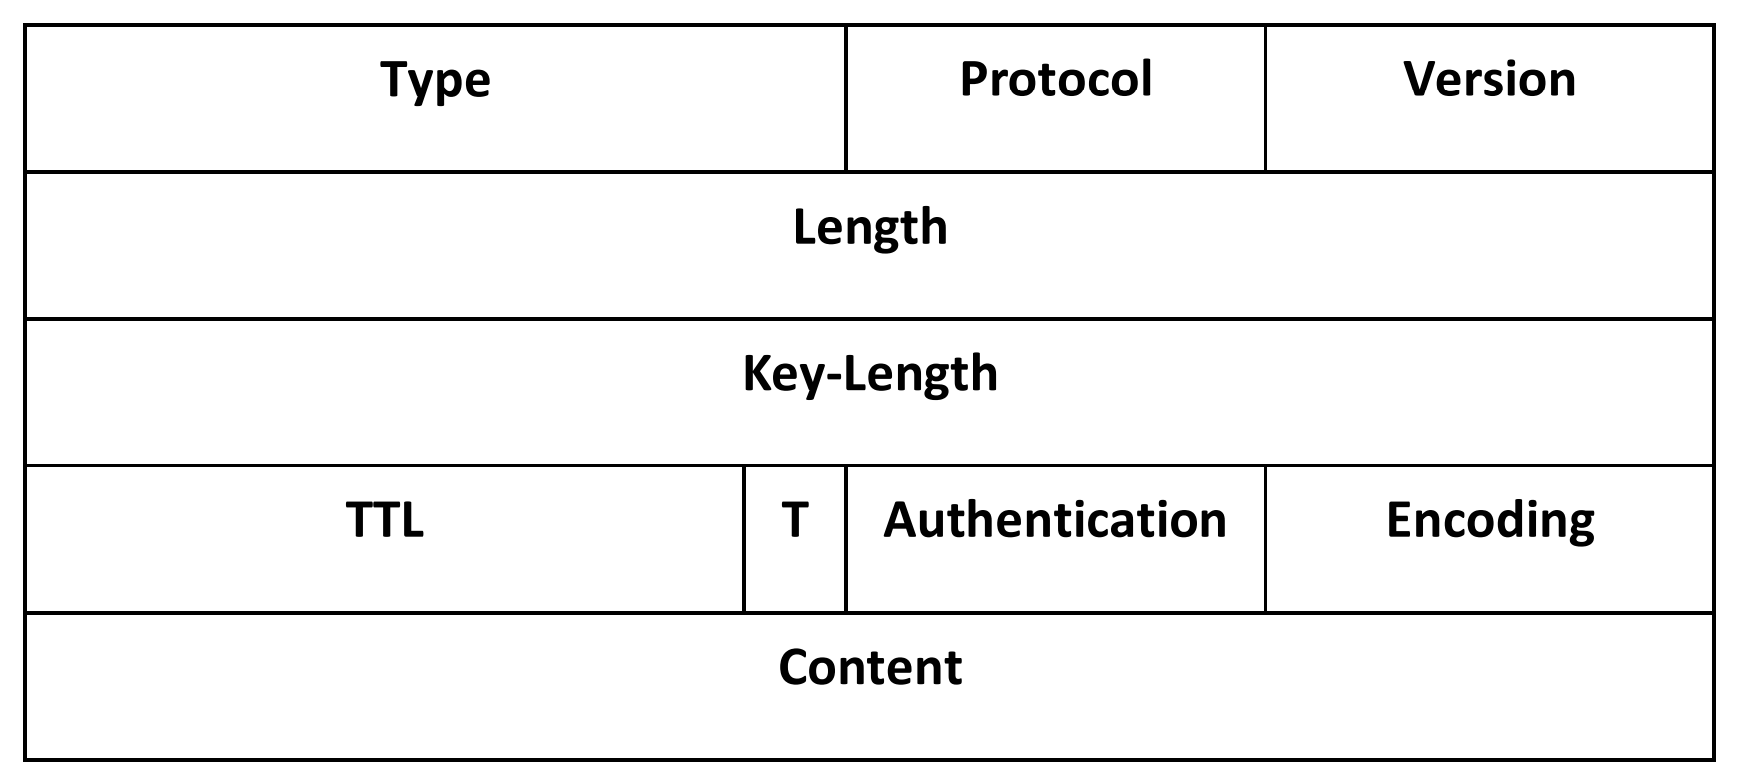
\includegraphics[width=0.8\textwidth]{MainContent/img/cap3/QKD Configuration Protocol.png}
    \caption{Formato messaggi di QKD Configuration Protocol}
    \label{fig:QKD_conf}
\end{figure}

\subsection{Quantum TLS Handshake Protocol}
Nello schema di TLS sono state introdotte alcune modifiche al protocollo di Handshake, in particolare la procedura classica di scambio delle chiavi (DH, RSA) è stata sostituita con il meccanismo di QKD utilizzando il protocollo BB84. Per questo motivo, verrà rinominato \textbf{Quantum TLS Handshake} . La Figura sottostante mostra i diversi messaggi inviati in questo protocollo.
\begin{figure}[H]
    \centering
    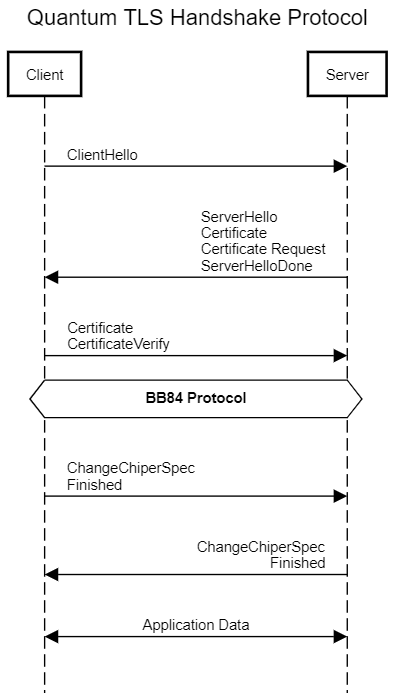
\includegraphics[width=0.5\textwidth]{MainContent/img/cap3/BB84diagram.png}
    \caption{Quantum TLS Handshake Protocol}
    \label{fig:QTLSHP}
\end{figure}
\noindent È possibile notare come il protocollo quantico BB84 sia integrato nell'handshake TLS. Inizialmente è presente una fase di autenticazione, in cui il Client ed il Server si autenticano reciprocamente scambiandosi i certificati. Una volta conclusa questa fase, viene eseguito il protocollo quantico ed il numero di fotoni che deve essere trasmesso dipende dalla lunghezza della chiave desiderata. Siccome BB84 è vulnerabile agli attacchi di tipo man-in-the-middle, una volta finita l’esecuzione del processo viene verificato se l’autenticazione è andata a buon fine.
\newpage

\subsection{Esempio di applicazione di questa soluzione QKD-TLS}
Per dimostrare l'effettiva applicabilità di questa soluzione, in questa sezione è presentato un esempio di implementazione di QKD-TLS \cite{laurenti_integration_nodate}. Consideriamo due reti LAN connesse da due modem ottici che giocano il ruolo di canale quantico e classico
allo stesso tempo. Il processo che permette di assicurare la sicurezza della connessione TLS tra Alice e Bob utilizzando il meccanismo di QKD è composto da cinque fasi:
\begin{figure}[H]
    \centering
    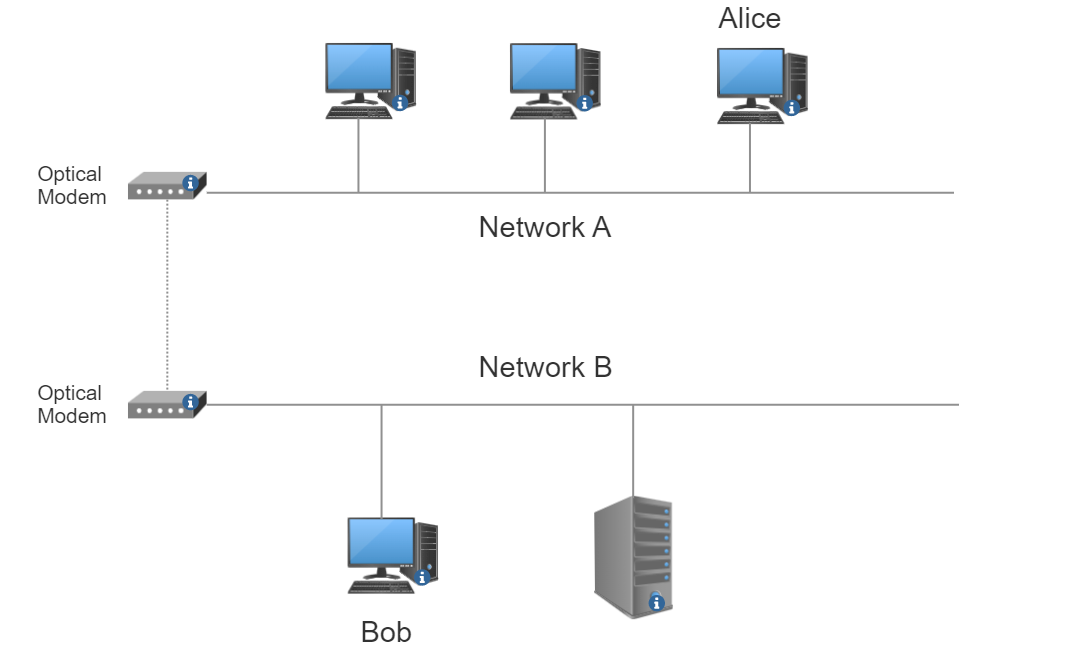
\includegraphics[width=0.8\textwidth]{MainContent/img/cap3/EsempioTLS.png}
    \caption{Esempio d’uso di due modem ottici in Quantum TLS}
    \label{fig:esempio}
\end{figure}

\begin{itemize}
    \item \textbf{Fase 1}: quando il TLS Record Protocol del nodo A, per esempio, prende i dati dal livello di applicazione, chiama il suo Application Data Protocol. Così i dati sono frammentati e per ogni frammento viene fatta una compressione.
    \item \textbf{Fase 2}: il TLS record Protocol chiama il QKD Configuration Protocol in modo che i nodi A e B si mettano d’accordo sui parametri del QKD Configuration Protocol illustrati in precedenza. I campi più importanti sono: \textit{protocol}, \textit{key - length} e i campi \textit{TTL} e \textit{T}. Nell’esempio scegliamo il protocollo BB84 perchè è il primo protocollo sperimentato ed è provata la sua sicurezza incondizionata. Assumiamo che non vi siano meccanismi di autenticazione e di codifica. Prendiamo in considerazione: \textit{Key - length} = 20 byte, \textit{TTL} = 200 messaggi, \textit{T} = 0. Nel caso in cui si volessimo utilizzare one-time-pad, per testare la sicurezza incondizionata dobbiamo scegliere \textit{TTL} = 1.
    
    \item \textbf{Fase 3}:  Il TLS Record Protocol usa il Quantum Handshake Protocol per ottenere i parametri di sicurezza. Così il Quantum Handshake Protocol viene eseguito e viene attuato il protocollo BB84 nei due modem. La chiave generata viene memorizzata in una memoria flash per essere usata più tardi nella codifica dal Record Protocol.
    
    \item \textbf{Fase 4}:Il TLS Record Protocol riceve la chiave fornita dal servizio QKD e costruisce i suoi parametri di sicurezza. Questi parametri sono usati per generare chiavi per codificare dati e assicurare l’integrità (MAC).
    
    \item \textbf{Fase 5}: una volta che il record (frammenti compressi, MAC e pudding opzionale) è stato criptato, al blocco appena codificato viene aggiunto un header e l’intero pacchetto viene passato al livello di trasporto.
\end{itemize}







